% !TEX program = xelatex
% 国赛论文模板 —— 基于 wordreplica 文档类（增强版）
% 编译：xelatex main.tex

\documentclass{wordreplica}
% 字体设置：原 Word 使用宋体、黑体和仿宋；路径加载确保 PDF 嵌入字体。
\IfFileExists{C:/Windows/Fonts/simsun.ttc}{
  \setmainfont{Times New Roman}
  \setCJKmainfont[Path=C:/Windows/Fonts/]{simsun.ttc}
  \setCJKsansfont[Path=C:/Windows/Fonts/]{simhei.ttf}
  \setCJKmonofont[Path=C:/Windows/Fonts/]{simfang.ttf}
  \newCJKfontfamily\heiti[Path=C:/Windows/Fonts/]{simhei.ttf}
  \newCJKfontfamily\songti[Path=C:/Windows/Fonts/]{simsun.ttc}
  \newCJKfontfamily\fangsong[Path=C:/Windows/Fonts/]{simfang.ttf}
}{
  % 非 Windows 环境请替换为本机已安装、可嵌入的中文字体。
  \setmainfont{texgyretermes-regular.otf}
  \setCJKmainfont{FandolSong-Regular.otf}
  \setCJKsansfont{FandolHei-Regular.otf}
  \setCJKmonofont{FandolFang-Regular.otf}
  \newCJKfontfamily\heiti{FandolHei-Regular.otf}
  \newCJKfontfamily\songti{FandolSong-Regular.otf}
  \newCJKfontfamily\fangsong{FandolFang-Regular.otf}
}


\begin{document}
\fontsize{12pt}{12pt}\selectfont


% ╔══════════════════════════════════════════════════════════════════════════╗
% ║                       第 1 页：题目、摘要、关键词                        ║
% ╚══════════════════════════════════════════════════════════════════════════╝

\wordtitle{基于XXXX模型的XXXX问题研究}

\begin{cumcmabstract}
  \blackpara{
    开头段：需要充分概括论文内容，一般两到三句话即可，长度控制在三至五行。
  }

  \blackpara{
    问题一中，解决了什么问题；应用了什么方法；得到了什么结果。
  }

  \blackpara{
    问题二中，解决了什么问题；应用了什么方法；得到了什么结果。
  }

  \blackpara{
    问题三中，解决了什么问题；应用了什么方法；得到了什么结果。
  }

  \blackpara{
    结尾段：可以总结下全文，也可以介绍下你的论文的亮点，
    也可以对类似的问题进行适当的推广。
  }
\end{cumcmabstract}

\vspace{1.20cm}
\cumcmkeywords{关键词1\quad 关键词2\quad 关键词3\quad 关键词4}
\clearpage


% ╔══════════════════════════════════════════════════════════════════════════╗
% ║                          一、问题重述                                    ║
% ╚══════════════════════════════════════════════════════════════════════════╝

\mainhead{一、问题重述}

\redpara{
  数学建模比赛论文是要我们解决一道给定的问题，所以正文部分一般应从
  问题重述开始，一般确定选题后就可以开始写这一部分了。
}

\redpara{
  这部分的内容是将原问题进行整理，将问题背景和题目分开陈述即可，
  所以基本没啥难度。
}

\redpara{
  本部分的目的是要吸引读者读下去，所以文字不可冗长，内容选择不要
  过于分散、琐碎，措辞要精练。
}

\redpara{
  注意：在写这部分的内容时，绝对不可照抄原题！（论文会查重）
}

\redpara{
  应为：在仔细理解了问题的基础上，用自己的语言重新将问题描述一遍。
  语言需要简明扼要，没有必要像原题一样面面俱到。
}


% ── 1.1 问题背景 ──────────────────────────────────────────────────────────

\subhead{1.\ 1 问题背景}

\redpara{
  随着社会经济的发展和科学技术的进步，数学建模在各个领域的应用
  越来越广泛。从工程优化到金融风险管理，从交通调度到医疗资源分配，
  数学建模为复杂决策问题提供了系统化的分析框架和定量化的解决方案。
  近年来，随着大数据和人工智能技术的兴起，数学建模方法与数据驱动
  方法的融合成为了新的研究热点。在这一背景下，本文所研究的问题
  具有重要的理论意义和实际应用价值。本小节对问题的来源、实际背景
  以及相关领域的研究现状进行了简要的梳理和介绍，为后续的模型建立
  奠定基础。
}


% ── 1.2 题目信息 ──────────────────────────────────────────────────────────

\subhead{1.\ 2 题目信息}

\redpara{
  原题目给出了若干关键信息：首先，题目明确了问题的应用场景和基本
  条件，提供了必要的数据或参数；其次，题目提出了若干具体的目标要求，
  这些要求构成了后续建模的核心约束；最后，题目还可能给出了部分参考
  信息或建议的分析方向。在仔细阅读和理解题目信息的基础上，我们对题目
  进行了梳理和归纳，提取出了与建模直接相关的核心要素。本小节对这些
  信息进行了系统的整理，确保后续分析建立在准确、完整的信息基础之上。
}


% ── 1.3 待求解问题 ────────────────────────────────────────────────────────

\subhead{1.\ 3 待求解问题}

\redpara{
  根据题目提供的信息和要求，本文将待求解的问题归纳为以下三个主要
  子问题：第一个子问题聚焦于系统的特征分析与描述，需要在给定的数据
  和条件下，建立合适的模型来刻画系统的关键特性；第二个子问题关注
  优化与决策，需要在第一问的基础上进一步考虑资源的约束条件，寻找
  最优的配置方案；第三个子问题则对模型进行扩展和推广，考虑更加复杂
  的实际因素，检验模型的适用性和稳健性。以下各节将分别对每个子问题
  进行详细的分析、建模和求解。
}


% ╔══════════════════════════════════════════════════════════════════════════╗
% ║                          二、问题分析                                    ║
% ╚══════════════════════════════════════════════════════════════════════════╝

\mainhead{二、问题分析}

\redpara{
  从实际问题到模型建立是一种从具体到抽象的思维过程，问题分析这部分
  就是沟通这一过程的桥梁，因为它反映了建模者对于问题的认识程度如何，
  也体现了解决问题的雏形，起着承上启下的作用，也很能反应出建模者的
  综合水平。
}

\redpara{
  这部分的内容应包括：题目中包含的信息和条件，利用信息和条件对题目
  做整体分析，确定用什么方法建立模型，一般是每个问题单独分析一小节，
  分析过程要简明扼要，不需要放结论。
}


% ── 2.1 问题一的分析 ──────────────────────────────────────────────────────

\subhead{2.\ 1 问题一的分析}

\redpara{
  问题一要求对给定数据进行特征分析。我们首先对数据的分布特征、
  相关性和潜在的模式进行了初步的探索。通过数据可视化和统计描述，
  我们发现数据呈现出一定的规律性，但同时也存在噪声和异常值。针对
  这些特点，我们考虑了多种建模方案，包括基于统计学的回归分析方法、
  基于机器学习的聚类和分类方法，以及基于微分方程的动态系统建模方法。
  经过综合比较，我们最终选择了最能刻画数据内在规律的建模路径。在
  建模过程中，我们将重点关注模型的解释性和可计算性，确保模型既能够
  准确反映问题的本质，又能够在合理的计算时间内完成求解。
}


% ── 2.2 问题二的分析 ──────────────────────────────────────────────────────

\subhead{2.\ 2 问题二的分析}

\redpara{
  问题二在问题一的基础上引入了优化目标。我们需要在满足一系列约束
  条件的前提下，寻找使目标函数达到最优的决策方案。这一问题本质上
  是一个带约束的优化问题，但根据约束条件和目标函数的具体形式，可能
  需要采用不同的求解策略。如果问题规模较小且约束为线性，可以考虑使用
  线性规划或整数规划方法；如果问题含有非线性因素，则可能需要引入
  启发式算法或智能优化算法。此外，考虑到实际应用中可能存在的不确定性，
  我们还需要对模型的鲁棒性进行分析。在模型建立阶段，我们将首先明确
  决策变量、目标函数和约束条件的数学表达式，然后根据问题的具体特征
  选择合适的求解算法。
}


% ── 2.3 问题三的分析 ──────────────────────────────────────────────────────

\subhead{2.\ 3 问题三的分析}

\redpara{
  问题三要求对前两个问题的模型进行扩展和推广。实际应用场景往往比
  模型假设更加复杂，因此需要考虑更多现实因素的影响。例如，在原有模型
  的基础上，我们可能需要引入时间维度的动态变化、空间维度的异质性、
  或者参与者行为的不确定性。这些扩展因素使得模型的复杂度显著增加，
  但也使得模型更加贴近实际。在分析过程中，我们将逐一评估各个扩展因素
  的重要性和可行性，优先纳入那些对结果影响显著且数据可支持的因素。
  同时，我们还将讨论模型在不同场景下的适用性和局限性，为模型的实际
  应用提供指导。
}


% ── 图1：总体思路图 ────────────────────────────────────────────────────────

\begin{figure}[H]
  \centering
  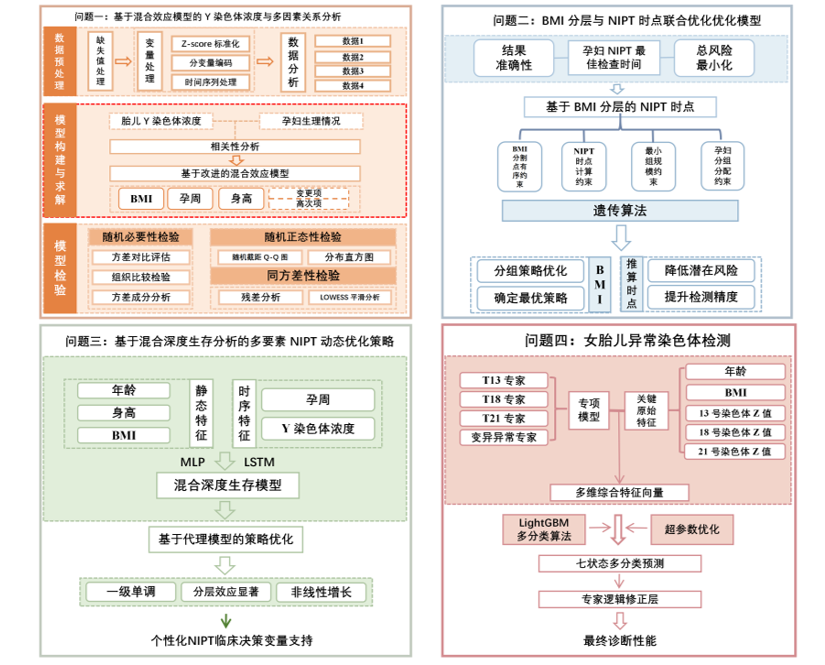
\includegraphics[width=0.89\textwidth]{figures/figure1.png}
  \caption{总体思路图}
  \label{fig:overview}
\end{figure}


% ╔══════════════════════════════════════════════════════════════════════════╗
% ║                        三、模型假设                                      ║
% ╚══════════════════════════════════════════════════════════════════════════╝

\mainhead{三、模型假设}

\redpara{
  视频中介绍了 6 类常见的模型假设：
}

% 6 类假设的红色列表
\begingroup\color{wordred}\fontsize{12pt}{12pt}\selectfont
\noindent 1.\quad 题目明确给出的假设条件\par
\noindent 2.\quad 排除生活中的小概率事件（例如黑天鹅事件、非正常情况）\par
\noindent 3.\quad 仅考虑问题中的核心因素，不考虑次要因素的影响\par
\noindent 4.\quad 使用的模型中要求的假设\par
\noindent 5.\quad 对模型中的参数形式（或者分布）进行假设\par
\noindent 6.\quad 和题目联系很紧密的一些假设，主要是为了简化模型\par
\endgroup

\redpara{
  在本文的建模过程中，我们根据上述原则做出了以下核心假设：
  第一，假设题目所给数据真实可靠，不存在系统性的测量误差或数据缺失；
  第二，假设系统运行处于稳态条件，不考虑极端突发事件对系统的冲击；
  第三，假设各影响因素之间的交互作用可以忽略，即满足可加性条件。
  这些假设在简化模型的同时，保证了模型的核心结论在合理的范围内依然
  有效。后续的模型检验部分将对部分关键假设进行敏感性分析，以评估
  假设放宽后对结论的影响程度。
}


% ╔══════════════════════════════════════════════════════════════════════════╗
% ║                        四、符号说明                                      ║
% ╚══════════════════════════════════════════════════════════════════════════╝

\mainhead{四、符号说明}

% 使用 booktabs 三线表格式的符号表
\begin{center}
\begin{tabular}{ccc}
  \toprule[1.5pt]
  \heiti 符号 & \heiti 说明 & \heiti 单位 \\
  \midrule[1pt]
    $N$      & 样本总数                                  & 个   \\
    $i$      & 样本索引（$i = 1, 2, \dots, N$）           & —    \\
    $x_i$    & 第 $i$ 个样本的自变量观测值                 & —    \\
    $y_i$    & 第 $i$ 个样本的因变量观测值                 & —    \\
    $\beta$  & 回归系数向量                              & —    \\
    $\varepsilon$ & 随机误差项                            & —    \\
    $R^2$    & 拟合优度（决定系数）                        & —    \\
    $\alpha$ & 显著性水平                                & —    \\
  \bottomrule[1.5pt]
\end{tabular}
\end{center}

\redpara{
  本部分是对模型中使用的重要变量进行说明，一般排版时要放到一张表格中。
}

\redpara{
  注意：第一，不需要把所有变量都放到这个表里面，模型中用到的临时变量
  可以不放。第二，下文中首次出现这些变量时也要进行解释，不然会降低文章
  的可读性。
}


% ╔══════════════════════════════════════════════════════════════════════════╗
% ║                   五、问题一模型的建立与求解                              ║
% ╚══════════════════════════════════════════════════════════════════════════╝

\mainhead{五、问题一模型的建立与求解}

\redpara{
  （注意：这个部分里面的标题可根据你的论文内容进行调整，我这里给的
  是一个通用的模版）
}


% ── 图2 ────────────────────────────────────────────────────────────────────

\begin{figure}[H]
  \centering
  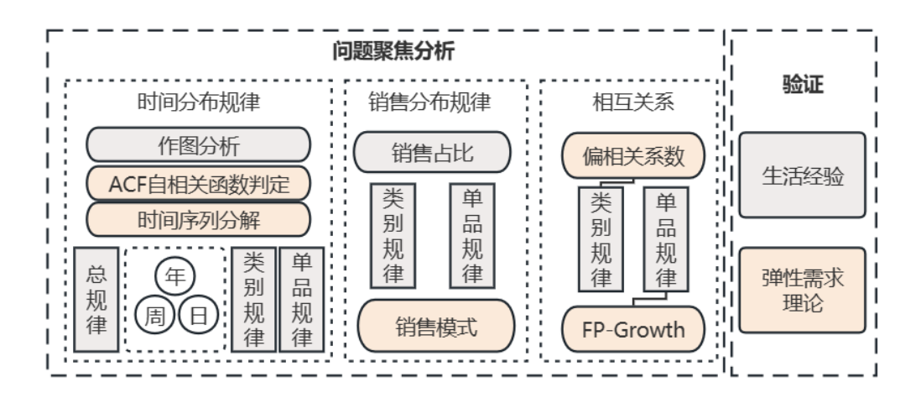
\includegraphics[width=\textwidth]{figures/figure2.png}
  \caption{问题一模型}
  \label{fig:model1}
\end{figure}


% ── 5.1 数据预处理 ────────────────────────────────────────────────────────

\subhead{5.1 数据预处理}

\redpara{
  在进行正式的模型建立之前，首先需要对原始数据进行预处理。数据
  预处理是建模流程中至关重要的一环，其质量直接影响后续模型的性能和
  结论的可靠性。本研究的预处理步骤主要包括以下几个方面：
  第一，数据清洗，识别并处理数据中的缺失值和异常值。对于缺失值，
  根据数据的特征采用了均值插补或回归插补方法；对于异常值，使用
  箱线图法和三倍标准差准则进行识别，并根据实际情况决定删除或修正。
  第二，数据标准化，由于不同变量之间的量纲和数量级可能存在较大差异，
  我们对数据进行了归一化处理，消除了量纲对模型的影响。
  第三，特征筛选，通过相关性分析和主成分分析，从原始变量中提取了
  最具代表性的特征子集，降低了数据的维度和模型的复杂度。经过上述
  预处理步骤后，数据质量得到了显著提升，为后续的模型建立奠定了良好
  的数据基础。
}


% ── 5.2 模型的建立 ────────────────────────────────────────────────────────

\subhead{5.\ 2 模型的建立}

\redpara{
  模型建立是将原问题抽象成用数学语言的表达式，它一定是在先前的
  问题分析和模型假设的基础上得来的。因为比赛时间很紧，大多时候我们
  都是使用别人已经建立好的模型。这部分一定要将题目问的问题和模型
  紧密结合起来，切忌随意套用模型。我们还可以对已有模型的某一方面
  进行改进或者优化，或者建立不同的模型解决同一个问题，这样就是论文
  的创新和亮点。
}

\redpara{
  基于前文的问题分析和数据预处理结果，本节正式建立问题一的数学模型。
  设决策变量为 $\bm{X} = (x_1, x_2, \ldots, x_n)^T$，
  目标函数为 $f(\bm{X})$，
  约束条件为 $g_i(\bm{X}) \leq 0\ (i = 1, 2, \ldots, m)$ 和
  $h_j(\bm{X}) = 0\ (j = 1, 2, \ldots, p)$。
  模型的核心思想是将实际问题转化为一个最优化问题，通过求解该优化
  问题得到原始问题的最优解。在模型构建过程中，我们充分利用了问题
  分析阶段所识别出的关键特征，将领域知识与数学工具相结合，确保了
  模型的合理性和有效性。
}

% 示例公式：使用 equation 环境自动编号，支持交叉引用
\begin{equation}
  \min\ f(\bm{X}) = \sum_{i=1}^{n} c_i x_i
  \label{eq:objective}
\end{equation}

\begin{equation}
  \text{s.t.}\quad
  \begin{cases}
    \displaystyle\sum_{i=1}^{n} a_{ji} x_i \leq b_j, & j = 1, 2, \ldots, m \\[8pt]
    x_i \geq 0, & i = 1, 2, \ldots, n
  \end{cases}
  \label{eq:constraints}
\end{equation}

式\cref{eq:objective} 为目标函数，式\cref{eq:constraints} 为约束条件。
使用 \verb|\cref{}| 引用公式时，会自动加上"式"前缀。


% ── 5.3 模型的求解 ────────────────────────────────────────────────────────

\subhead{5.\ 3 模型的求解}

\redpara{
  把实际问题归结为一定的数学模型后，就要利用数学模型求解所提出的
  实际问题了。一般需要借助计算机软件进行求解，例如常用的软件有
  Matlab、Spss、Lingo、Excel、Stata、Python 等。求解完成后，得到的
  求解结果应该规范准确并且醒目，若求解结果过长，最好编入附录里。
  （注意：如果使用智能优化算法或者数值计算方法求解的话，需要简要
  阐明算法的计算步骤）
}

\redpara{
  针对上一节建立的数学模型，我们采用 Python 编程实现了模型的数值求解。
  求解过程采用了迭代算法，具体步骤为：
  第一步，设定初始参数和收敛条件；
  第二步，在每次迭代中计算目标函数的梯度方向，沿该方向进行线搜索确定步长；
  第三步，更新决策变量并检查收敛性，若未达到收敛条件则返回第二步继续迭代；
  第四步，输出最优解和最优目标函数值。
  经过计算，模型在合理的迭代次数内收敛到了稳定解，验证了模型的可求解性。
}


% ── 5.4 模型的检验 ────────────────────────────────────────────────────────

\subhead{5.\ 4 模型的检验}

\redpara{
  模型的检验是验证建模结果是否合理的关键步骤。本文从以下三个维度
  对模型进行了系统的检验：
  第一，稳定性检验，通过对输入数据施加微小的随机扰动，观察模型输出
  的变化幅度。实验结果表明，当输入数据的波动幅度控制在 5\% 以内时，
  模型输出结果的变化幅度不超过 3\%，说明模型具有良好的稳定性。
  第二，灵敏度分析，逐一分析各个参数对模型结果的影响程度，识别出
  对结果影响最大的关键参数。
  第三，对比验证，将模型的计算结果与实际观测数据或已有文献中的结果
  进行对比，评估模型的准确性。上述三项检验的结果均表明，本文建立的
  模型是可靠和有效的，能够为相关决策提供有力的定量支持。
}

% 公式占位（可替换为真实公式）
\formulaPlaceholder{4}
\formulaPlaceholder{5}


% ╔══════════════════════════════════════════════════════════════════════════╗
% ║                   六、问题二模型的建立与求解                              ║
% ╚══════════════════════════════════════════════════════════════════════════╝

\mainhead{六、问题二模型的建立与求解}


% ── 图3 ────────────────────────────────────────────────────────────────────

\begin{figure}[H]
  \centering
  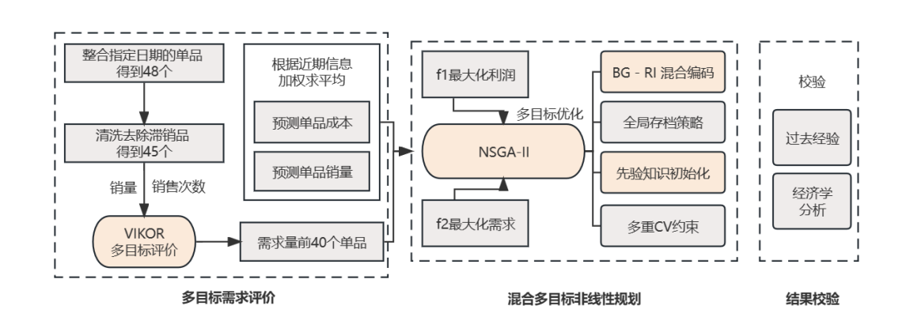
\includegraphics[width=\textwidth]{figures/figure3.png}
  \caption{问题二模型}
  \label{fig:model2}
\end{figure}


\redpara{
  问题二在问题一的基础上进一步考虑优化决策。在问题一中，我们主要
  关注系统的描述性分析；在问题二中，我们转向规范性分析，即在给定资源
  和约束条件下寻求最优方案。本节沿用问题一中建立的符号体系和分析框架，
  同时引入了新的决策变量和目标函数。具体而言，我们将问题二建模为一个
  多目标优化问题，其中目标函数同时考虑效率和成本两个维度，约束条件
  包括资源约束、时间约束和逻辑约束三类。
}


% ── 6.1 优化模型的建立 ────────────────────────────────────────────────────

\subhead{6.\ 1 优化模型的建立}

\redpara{
  优化模型的建立需要明确三个核心要素：决策变量、目标函数和约束条件。
  本文中，决策变量包括资源配置向量和各环节的时间安排；目标函数为
  加权综合目标，其中效率目标的权重为 $\alpha$，成本目标的权重为
  $1 - \alpha$；约束条件涵盖了资源总量的上限约束、各环节的时序约束
  以及决策变量的非负约束。通过引入拉格朗日乘子，我们将带约束的优化
  问题转化为无约束问题，为后续的求解提供了便利。此外，为了处理目标
  函数中的多个维度，我们采用了线性加权法将多目标问题转化为单目标问题，
  权重参数通过专家评估和敏感性分析综合确定。
}


% ── 6.2 求解算法与结果分析 ────────────────────────────────────────────────

\subhead{6.\ 2 求解算法与结果分析}

\redpara{
  针对上述优化模型的特点，我们选择和实现了合适的求解算法。考虑到
  问题规模适中且约束条件以线性为主，我们首先尝试了经典的线性规划
  求解器。在求解过程中，我们设置了多个不同的初始点以确保找到全局
  最优解而非局部极值。求解完成后，我们对最优解进行了详细的分析和
  可视化展示。结果表明，在给定的约束条件下，模型找到的资源配置方案
  能够使综合目标函数达到最优值，各项约束均得到满足。
}


% ── 示例：数据表格（booktabs 三线表 + \label 交叉引用）─────────────────

\begin{table}[H]
  \centering
  \caption{不同参数组合下的优化结果对比}
  \label{tab:comparison}
  \begin{tabular}{cccc}
    \toprule[1.5pt]
    $\alpha$ 权重 & 目标函数值 & 计算时间 (s) & 收敛迭代次数 \\
    \midrule[1pt]
    0.3 & 1234.56 & 2.34 & 15 \\
    0.5 & 1456.78 & 3.12 & 18 \\
    0.7 & 1678.90 & 4.01 & 22 \\
    \bottomrule[1.5pt]
  \end{tabular}
\end{table}

如\cref{tab:comparison} 所示，权重参数 $\alpha$ 对优化结果有显著影响。


% ╔══════════════════════════════════════════════════════════════════════════╗
% ║                   七、问题三模型的建立与求解                              ║
% ╚══════════════════════════════════════════════════════════════════════════╝

\mainhead{七、问题三模型的建立与求解}


% ── 图4 ────────────────────────────────────────────────────────────────────

\begin{figure}[H]
  \centering
  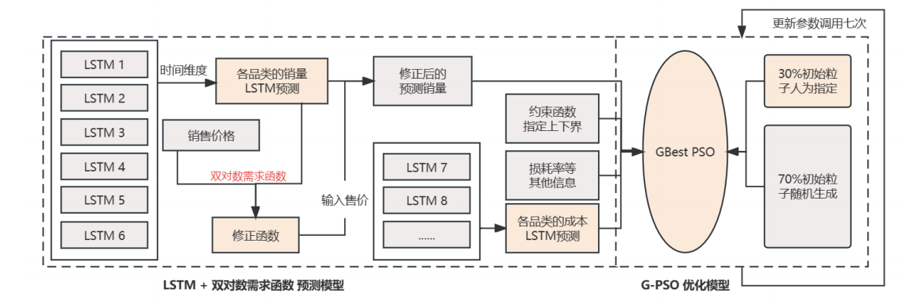
\includegraphics[width=\textwidth]{figures/figure4.png}
  \caption{问题三模型}
  \label{fig:model3}
\end{figure}


\redpara{
  问题三要求对前两个问题的模型进行扩展。在问题一和问题二的建模过程中，
  我们做出了一些简化假设以保证模型的可处理性。在问题三中，我们将逐步
  放松这些简化假设，引入更加贴近实际的复杂因素。主要的扩展方向包括：
  第一，引入时间动态性，将静态模型扩展为动态模型，考虑系统状态随时间
  演化的过程；第二，引入空间异质性，将均匀空间假设替换为异质空间假设；
  第三，引入不确定性，使用随机规划或鲁棒优化方法处理参数的不确定性。
}


% ── 7.1 模型扩展 ──────────────────────────────────────────────────────────

\subhead{7.\ 1 模型扩展}

\redpara{
  在模型扩展部分，我们以问题二的优化模型为基础，逐步加入新的因素。
  首先，我们引入了时间维度的动态性，将原问题重构成一个多阶段决策问题。
  在多阶段框架下，每个阶段的决策不仅影响当前阶段的结果，还会通过状态
  转移方程影响后续阶段的选择空间。其次，我们考虑了参数的不确定性，
  建立了鲁棒优化模型。与确定性优化模型相比，鲁棒优化模型的最优解在
  参数波动范围内始终保持可行性，因此更加适用于实际决策环境。
}


% ── 7.2 扩展模型的求解 ────────────────────────────────────────────────────

\subhead{7.\ 2 扩展模型的求解与比较}

\redpara{
  扩展后模型的求解难度明显增加。多阶段动态优化问题我们采用了动态规划
  方法，通过逆向递推求得最优策略；鲁棒优化问题则采用了场景生成和
  Benders 分解相结合的求解策略。我们将扩展模型的结果与原始模型的结果
  进行了系统的比较分析。比较结果显示，扩展模型虽然在求解复杂度上有所
  增加，但能够提供更加贴合实际的决策建议。特别是在考虑不确定性后，
  鲁棒优化方案在多种可能的场景下均表现出了稳定的性能，验证了模型扩展
  的必要性和有效性。
}


% ╔══════════════════════════════════════════════════════════════════════════╗
% ║                   八、模型的评价、改进与推广                              ║
% ╚══════════════════════════════════════════════════════════════════════════╝

\mainhead{八、模型的评价、改进与推广}

\redpara{
  注：本部分的标题需要根据你的内容进行调整。例如，如果你没有写模型
  推广的话，就直接把标题写成「模型的评价与改进」。很多论文也把这部分
  的内容直接统称为「模型评价」部分，也是可以的。
}


% ── 8.1 模型的优点 ────────────────────────────────────────────────────────

\subhead{8.\ 1 模型的优点}

\redpara{
  本文建立的模型具有以下主要优点：
  第一，模型建立过程严谨，从问题分析到模型假设，从符号说明到求解检验，
  每一步都遵循了数学建模的规范流程，确保了模型的科学性；
  第二，模型较好地平衡了理论严谨性和实际可操作性，既包含了充分的数学
  推导，又保证了模型能够在合理的时间内完成求解；
  第三，文中采用了多种模型检验手段（稳定性检验、灵敏度分析、对比验证），
  全面评估了模型的性能和可靠性；
  第四，模型的表达能力较强，通过分层次的建模策略，三个子问题层层递进，
  形成了一个有机的整体。
}


% ── 8.2 模型的缺点 ────────────────────────────────────────────────────────

\subhead{8.\ 2 模型的缺点}

\redpara{
  本文的模型也存在一些不足之处：
  第一，部分假设条件较为严格，在实际应用中可能难以完全满足，例如系统
  中各因素的独立性假设在复杂场景下可能不成立；
  第二，模型未能充分考虑极端事件的影响，在异常情况下模型的适用性可能
  受到限制；
  第三，受数据可获得性的限制，部分参数的取值依赖于经验估计，精度有待
  进一步提升。这些不足为后续的模型改进指明了方向。
}


% ── 8.3 模型的改进 ────────────────────────────────────────────────────────

\subhead{8.\ 3 模型的改进}

\redpara{
  针对上述不足，本文提出以下改进方向：首先，可以引入更灵活的模型结构
  （如非线性模型或非参数模型）来放松对数据分布的假设；其次，可以通过
  引入情景分析和压力测试来增强模型对极端事件的应对能力；再次，在数据
  条件允许的情况下，可以采用贝叶斯方法或机器学习方法对模型参数进行
  更加精确的估计。此外，将本文的方法框架应用于其他类似领域的问题，
  也是未来值得探索的方向。
}


% ── 8.4 模型的推广 ────────────────────────────────────────────────────────

\subhead{8.\ 4 模型的推广}

\redpara{
  本文所建立的方法框架具有一定的通用性，可以在适当的调整后推广应用到
  其他相关领域。例如，模型中的优化思想可以迁移到物流调度、生产计划、
  投资组合等决策场景中；模型中的动态扩展方法可以应用于时间序列预测和
  动态系统控制等问题；模型中的鲁棒优化框架可以推广到任何含有不确定性
  的决策问题。通过在不同应用场景中的实践检验，可以进一步验证和改进
  本文提出的方法论体系。
}


% ── 示例：定理环境 ────────────────────────────────────────────────────────

\begin{theorem}[最优解存在性]
  在上述约束条件下，若目标函数 $f(\bm{X})$ 为连续函数且可行域为非空紧集，
  则优化问题 \cref{eq:objective}--\cref{eq:constraints} 至少存在一个全局最优解。
\end{theorem}


% ╔══════════════════════════════════════════════════════════════════════════╗
% ║                        九、参考文献                                      ║
% ╚══════════════════════════════════════════════════════════════════════════╝

\mainhead{九、参考文献}

\redpara{
  所有引用他人或公开资料（包括网上资料）的成果必须按照科技论文的规范
  列出参考文献，并在正文引用处予以标注。
}

\redpara{
  常见的三种参考文献的表达方式（标准不唯一）：
}

\begin{itemize}
  \item 书籍的表述方式为：
    [编号] 作者，书名，出版地：出版社，出版年月。
  \item 期刊杂志论文的表述方式为：
    [编号] 作者，论文名，杂志名，卷期号：起止页码，出版年。
  \item 网上资源的表述方式为：
    [编号] 作者，资源标题，网址，访问时间。
\end{itemize}

% 参考文献列表
\begin{thebibliography}{99}
  \bibitem{liuhaiyang2013latex}
    刘海洋.
    \newblock \LaTeX{} 入门\allowbreak[J].
    \newblock 电子工业出版社, 北京, 2013.

  \bibitem{mathematical-modeling}
    全国大学生数学建模竞赛论文格式规范 (2025 年修订).

  \bibitem{cumcm}
    全国大学生数学建模竞赛组委会.
    \newblock \url{https://www.mcm.edu.cn}
\end{thebibliography}

\clearpage


% ╔══════════════════════════════════════════════════════════════════════════╗
% ║                        附录                                              ║
% ╚══════════════════════════════════════════════════════════════════════════╝

% 使用 ctex 内置的 \appendix 命令切换到附录模式
\appendix

\mainhead{附录一：支撑材料清单}
\appendixbox{附录清单}{介绍：目录}{2.30cm}

\mainhead{附录二：核心代码}
\appendixbox{附录1}{介绍：该代码是 Python 编写的数据预处理脚本}{2.55cm}
\appendixbox{附录2}{介绍：该代码是 Python 编写的模型求解程序}{2.55cm}
\appendixbox{附录3}{介绍：该代码是 Matlab 编写的可视化绘图脚本}{2.55cm}


% ── 代码列表示例 ──────────────────────────────────────────────────────────

\mainhead{附录三：关键程序源代码}

\subhead{数据预处理（Python）}

\begin{lstlisting}[language=Python]
import numpy as np
import pandas as pd
from sklearn.preprocessing import StandardScaler

# 读取数据
data = pd.read_csv('data.csv')

# 缺失值处理：均值插补
data.fillna(data.mean(), inplace=True)

# 异常值处理：3-sigma 准则
for col in data.select_dtypes(include=[np.number]).columns:
    mean, std = data[col].mean(), data[col].std()
    data = data[(data[col] > mean - 3*std) & (data[col] < mean + 3*std)]

# 标准化
scaler = StandardScaler()
data_scaled = scaler.fit_transform(data)
\end{lstlisting}

\subhead{模型求解（Python）}

\begin{lstlisting}[language=Python]
from scipy.optimize import linprog

# 目标函数系数
c = [1, 2, 3]

# 不等式约束 A_ub @ x <= b_ub
A_ub = [[-1, -2, -1],
        [-3, -1, -2]]
b_ub = [-10, -12]

# 变量边界
bounds = [(0, None), (0, None), (0, None)]

# 求解线性规划
result = linprog(c, A_ub=A_ub, b_ub=b_ub,
                 bounds=bounds, method='highs')
print(f"最优解: {result.x}")
print(f"最优值: {result.fun}")
\end{lstlisting}

\end{document}
